% !TEX program = xelatex
\documentclass[UTF8,zihao=-4]{ctexart}

% ---------- 页面与常用宏包 ----------
\usepackage[a4paper,top=2.8cm,bottom=2.4cm,left=2.4cm,right=2.4cm,headheight=28pt,headsep=0.7cm]{geometry}
\usepackage{graphicx}
\usepackage{xcolor}
\usepackage{fancyhdr}
\usepackage{lastpage}
\usepackage{titlesec}
\usepackage{booktabs}
\usepackage{array}
\usepackage{float}
\usepackage{caption}
\usepackage{listings}
\usepackage{hyperref}
\usepackage{enumitem}
\usepackage{amsmath,amssymb}
\usepackage{adjustbox}

\graphicspath{{lab6_report_assets/}}

\hypersetup{
  colorlinks=true,
  linkcolor=black,
  urlcolor=blue,
  citecolor=black
}

\setlength{\parindent}{2em}
\linespread{1.25}

% ---------- 基本信息 ----------
\newcommand{\CourseName}{CS2306}
\newcommand{\ReportTitle}{Lab6}
\newcommand{\ReportSubtitle}{简单的类 MIPS 多周期流水化处理器实现}
\newcommand{\StudentName}{姓名：\underline{\makebox[5cm][c]{吴恒涛}}}
\newcommand{\StudentID}{学号：\underline{\makebox[5cm][c]{524031910038}}}

% ---------- 页眉 SJTU logo ----------
\newcommand{\SJTUHeaderLogo}{%
  \IfFileExists{sjtu-logo.png}
  {
\includegraphics[height=0.85cm]{sjtu-logo.png}}
  {\fbox{\parbox[c][0.65cm][c]{2.6cm}{\centering\scriptsize SJTU LOGO}}}%
}

\pagestyle{fancy}
\fancyhf{}
\fancyhead[L]{\SJTUHeaderLogo}
\fancyhead[R]{\small\bfseries \CourseName\ \ReportTitle：\ReportSubtitle}
\fancyfoot[C]{第 \thepage\ 页 共 \pageref{LastPage} 页}
\renewcommand{\headrulewidth}{0.5pt}
\renewcommand{\footrulewidth}{0pt}

\fancypagestyle{plain}{%
  \fancyhf{}
  \fancyhead[L]{\SJTUHeaderLogo}
  \fancyhead[R]{\small\bfseries \CourseName\ \ReportTitle：\ReportSubtitle}
  \fancyfoot[C]{第 \thepage\ 页 共 \pageref{LastPage} 页}
  \renewcommand{\headrulewidth}{0.5pt}
}

% ---------- 标题格式 ----------
\titleformat{\section}{\zihao{3}\bfseries}{\thesection}{0.8em}{}
\titleformat{\subsection}{\zihao{4}\bfseries}{\thesubsection}{0.8em}{}
\titleformat{\subsubsection}{\bfseries}{\thesubsubsection}{0.8em}{}

% ---------- 代码格式 ----------
\definecolor{codegray}{RGB}{245,245,245}
\definecolor{codered}{RGB}{180,40,60}
\definecolor{codeblue}{RGB}{30,80,150}

\lstdefinestyle{mystyle}{
  backgroundcolor=\color{codegray},
  basicstyle=\ttfamily\small,
  keywordstyle=\color{codeblue}\bfseries,
  commentstyle=\color{gray},
  stringstyle=\color{codered},
  numbers=none,
  breaklines=true,
  frame=single,
  rulecolor=\color{black!30},
  tabsize=2,
  showstringspaces=false
}
\lstset{style=mystyle}

\begin{document}

% ---------- 封面 ----------
\begin{titlepage}
  \thispagestyle{plain}
  \centering
  \vspace*{2.2cm}
  {\zihao{1}\bfseries \ReportTitle\par}
  \vspace{0.6cm}
  {\zihao{2}\bfseries \ReportSubtitle\par}
  \vspace{1.2cm}
  {\zihao{3}\CourseName\par}
  \vfill
  \begin{tabular}{c}
    \zihao{4}\StudentName \\[1.0em]
    \zihao{4}\StudentID \\[1.0em]
    \zihao{4}日期：\underline{\makebox[5cm][c]{\today}}
  \end{tabular}
  \vfill
\end{titlepage}

\begin{abstract}
本次实验在 Lab5 单周期 CPU 的基础上实现了一个简单的类 MIPS 五级流水处理器。设计将指令执行过程划分为 IF、ID、EX、MEM、WB 五个阶段，并通过 IF/ID、ID/EX、EX/MEM、MEM/WB 四组流水寄存器保存阶段间的数据与控制信号。在基本流水线能够正确执行的基础上，进一步加入 Forwarding 机制解决普通 Read-After-Write 数据相关，加入 Stall 机制处理 \texttt{lw} 指令引起的 load-use 冒险，并通过 Flush 清除分支和寄存器跳转造成的错误取指。最后，结合补充实验，对 31 条指令扩展工程进行了单独测试。仿真结果表明，基础测试中的关键寄存器结果符合预期，Stall、Forwarding 和 Flush 均能在对应场景下生效；31 条指令扩展测试也能够跑通并得到正确的寄存器变化。
\end{abstract}

\tableofcontents
\newpage

\section{实验目标}

本实验的目标是将已经完成的类 MIPS 单周期 CPU 改造成五级流水 CPU，并在此基础上补充必要的冒险处理机制。具体来说，需要完成以下工作：

\begin{enumerate}[label=\arabic*.]
  \item 理解流水线处理器的基本执行方式，将一条指令的执行过程拆分为 IF、ID、EX、MEM、WB 五个阶段。
  \item 在相邻阶段之间加入流水寄存器，使指令、PC、操作数、立即数、目标寄存器号和控制信号能够随指令逐级传递。
  \item 完成基础流水线数据通路，使不含复杂相关的测试程序能够正常取指、译码、执行、访存和写回。
  \item 实现 Forwarding 机制，将 EX/MEM 或 MEM/WB 阶段已经得到的结果前递到 EX 阶段，减少普通数据相关带来的等待。
  \item 实现 Stall 机制，对 \texttt{lw} 后立即使用结果的 load-use 冒险插入一个气泡，避免后一条指令过早进入 EX 阶段。
  \item 实现 Flush 机制，在分支成立或 \texttt{jr} 跳转时清除错误路径上的指令。
  \item 完成 31 条指令扩展部分的补充验证，说明新增指令在流水线结构下能够正确执行。
\end{enumerate}

与 Lab5 相比，本实验的重点已经不只是单条指令能否得到正确结果，而是多条指令同时存在于流水线中时，数据、控制信号和 PC 更新能否保持一致。因此，报告中重点说明流水寄存器、冒险检测、前递选择和控制冒险处理这几个部分。

\section{总体设计思路}

\subsection{五级流水阶段划分}

单周期 CPU 中，一条指令需要在一个时钟周期内完成取指、译码、执行、访存和写回。流水化以后，这五个步骤被拆分到不同阶段中执行，多条指令可以在同一时刻处于不同阶段。这样可以提高处理器吞吐率，但也要求每一级的输入在当前周期内保持稳定，并且要求控制信号必须跟随对应指令向后传播。

本实验采用的五级流水结构如表~\ref{tab:stage} 所示。

\begin{table}[H]
  \centering
  \caption{五级流水阶段划分}
  \label{tab:stage}
  \begin{tabular}{c c p{8.5cm}}
    \toprule
    阶段 & 名称 & 主要功能 \\
    \midrule
    IF & Instruction Fetch & 根据 PC 从指令存储器取出当前指令，同时计算 PC+4，作为下一条顺序指令地址和部分跳转指令的返回地址基础。\\
    ID & Instruction Decode & 对指令进行译码，读取寄存器堆，生成立即数扩展结果和控制信号，同时初步判断部分控制流指令。\\
    EX & Execute & 根据 ALU 控制信号完成算术逻辑运算、移位、比较和访存地址计算，也是普通数据前递的主要使用阶段。\\
    MEM & Memory Access & 对数据存储器进行读写，主要服务于 \texttt{lw} 和 \texttt{sw} 指令。\\
    WB & Write Back & 选择 ALU 结果、内存读数或返回地址，将最终结果写回寄存器堆。\\
    \bottomrule
  \end{tabular}
\end{table}

流水化以后，一条指令不再一次性经过完整数据通路，而是在每个周期只完成其中一个阶段。因此，顶层模块不仅要连接原有的 ALU、寄存器堆和存储器，还要在阶段之间加入状态保存逻辑。这样后一级使用的是前一周期传来的旧指令信息，而不是当前 ID 阶段正在译码的新指令信息。

\subsection{工程模块组织}

本实验保留了 Lab5 中已经完成的基础模块，包括指令存储器、寄存器堆、ALU、数据存储器、符号扩展、零扩展和 ALU 控制单元。在此基础上，重新组织 Top 模块，并新增流水寄存器和冒险处理相关模块。整体分工如下：

\begin{itemize}
  \item \texttt{Top.v}：负责五级流水数据通路的连接，集中处理 PC 更新、写回反馈、前递输入选择、Stall 和 Flush。
  \item \texttt{if\_id.v}：保存 IF 阶段取出的指令和 PC+4，并对 Stall 和 Flush 做特殊处理。
  \item \texttt{id\_ex.v}：保存 ID 阶段产生的寄存器读数、扩展结果、寄存器编号和后续控制信号。
  \item \texttt{ex\_mem.v}：保存 EX 阶段产生的 ALU 结果、写内存数据、目标寄存器号和访存/写回控制信号。
  \item \texttt{mem\_wb.v}：保存 WB 阶段写寄存器所需的写回数据、目标寄存器号和写使能。
  \item \texttt{forwarding.v}：判断 EX 阶段的两个 ALU 输入是否需要来自 MEM 或 WB 阶段的前递数据。
  \item \texttt{hazard\_detection.v}：检测 load-use 冒险，并产生 Stall 信号。
\end{itemize}

为了避免信号命名混乱，我在顶层中按照流水阶段给中间信号加前缀。例如 \texttt{IF\_instr} 表示 IF 阶段取出的指令，\texttt{ID\_instr} 表示 IF/ID 流水寄存器输出到 ID 阶段的指令，\texttt{EX\_alu\_result} 表示 EX 阶段 ALU 的计算结果。这种命名方式可以直接反映信号属于哪一级流水，有助于在波形中定位问题。

\subsection{流水化后需要额外解决的问题}

流水线 CPU 的主要困难不在于单个模块的功能，而在于不同指令之间的相互影响。结合本次实验，主要有以下三类问题：

\begin{enumerate}[label=\arabic*.]
  \item \textbf{控制信号错位问题}：控制信号在 ID 阶段生成，但真正使用它们的阶段可能是 EX、MEM 或 WB。如果不把控制信号写入流水寄存器，后级可能会错误使用当前指令的新控制信号。
  \item \textbf{数据相关问题}：后一条指令可能需要使用前一条指令的计算结果，而此时结果尚未写回寄存器堆。普通 ALU 结果相关可以通过 Forwarding 解决，\texttt{lw} 后的 load-use 冒险则需要 Stall。
  \item \textbf{控制冒险问题}：分支或跳转改变 PC 时，流水线中可能已经取入错误路径上的指令。此时需要 Flush，防止错误指令继续写寄存器或写内存。
\end{enumerate}

\section{基础流水功能实现}

\subsection{IF 阶段与 PC 更新}

IF 阶段的主要任务是根据当前 PC 取出指令，并计算 PC+4。普通情况下，下一周期 PC 直接更新为 PC+4；当出现 Stall 时，PC 必须保持原值；当出现分支成立或 \texttt{jr} 跳转时，PC 需要更新为修正后的目标地址。

顶层中的 PC 更新逻辑可以概括为以下优先级：Reset 最高，Stall 用于冻结当前取指位置，Flush 或跳转用于修正 PC，其余情况按顺序执行。

\begin{lstlisting}[language=Verilog]
assign PC_add_4 = PC + 4;

assign renew_pc = ID_jr ? jr_targ :
                  (branch_taken ? branch_targ : PC_add_4);

always @(posedge Clk) begin
  if (Reset)
    PC <= 32'b0;
  else if (Stall)
    PC <= PC;
  else if (Flush)
    PC <= renew_pc;
  else
    PC <= PC_add_4;
end
\end{lstlisting}

这里需要注意，Stall 时只保持 PC 还不够，还必须配合 IF/ID 流水寄存器保持不变，否则 PC 虽然没有前进，但 ID 阶段的指令仍可能发生变化，导致同一条指令对应的数据和控制信号错位。

\subsection{IF/ID 流水寄存器}

IF/ID 流水寄存器保存两项核心内容：当前取出的指令和 PC+4。指令内容用于 ID 阶段译码，PC+4 后续可用于分支目标计算或 \texttt{jal} 返回地址。该寄存器也是 Stall 和 Flush 最先影响的流水寄存器。

\begin{lstlisting}[language=Verilog]
always @(negedge clock) begin
  if (flush) begin
    instr_buffer <= 32'b0;
    pc_buffer <= 32'b0;
  end
  else if (stall) begin
    instr_buffer <= instr_buffer;
    pc_buffer <= pc_buffer;
  end
  else begin
    instr_buffer <= if_instr;
    pc_buffer <= if_pc;
  end
end
\end{lstlisting}

当 \texttt{flush=1} 时，说明已经取入了错误路径上的指令，因此将指令清零，相当于向流水线中送入空操作。当 \texttt{stall=1} 时，说明 ID 阶段的指令暂时不能继续向后推进，因此 IF/ID 保持原值。正常情况下，IF 阶段的新指令进入 ID 阶段。

\subsection{ID/EX 流水寄存器}

ID/EX 流水寄存器保存的内容最多，因为 ID 阶段是控制信号和操作数集中产生的阶段。它需要把寄存器读数、立即数扩展结果、寄存器编号和多类控制信号一并送到 EX 阶段。

主要保存内容如下：

\begin{itemize}
  \item 两个寄存器读数 \texttt{reg\_data\_1} 和 \texttt{reg\_data\_2}；
  \item 符号扩展结果、零扩展结果以及移位量字段；
  \item \texttt{rs}、\texttt{rt}、\texttt{rd} 等寄存器编号，用于后续前递判断和写回目标选择；
  \item \texttt{ALUSrc}、\texttt{ALUOp}、\texttt{MemRead}、\texttt{MemWrite}、\texttt{MemToReg}、\texttt{RegWrite} 等控制信号。
\end{itemize}

在这里，目标寄存器号不能在 WB 阶段再临时判断，因为到 WB 阶段时原始指令字段已经不一定完整保留。更稳妥的做法是在 ID/EX 阶段就根据指令类型选出目标寄存器号，并随流水线向后传递。

\begin{lstlisting}[language=Verilog]
after_ext = sign_ext_buffer_sel ? signext_buffer : zeroext_buffer;

reg_dst = jump_load_buffer ? 5'b11111 :
          (reg_dst_buffer_sel ? reg_dst_index_buffer[4:0] :
                                reg_dst_index_buffer[9:5]);
\end{lstlisting}

其中 \texttt{jump\_load} 对应 \texttt{jal}，需要将返回地址写入 \$31；R 型指令写 \texttt{rd}，I 型指令写 \texttt{rt}。这个选择结果继续向 EX/MEM 和 MEM/WB 传递，保证最终写回目标与当前指令一致。

\subsection{EX/MEM 与 MEM/WB 流水寄存器}

EX/MEM 保存 ALU 结果、写内存数据、目标寄存器号和 MEM/WB 阶段需要的控制信号。对于 \texttt{lw} 和 \texttt{sw}，ALU 结果作为数据存储器地址；对于算术逻辑指令，ALU 结果最终会被写回寄存器堆。\texttt{sw} 还需要把第二个寄存器读数作为写内存数据继续向后传递。

MEM/WB 保存最后写回阶段需要的内容。写回数据可能来自数据存储器，也可能来自 ALU。具体选择由 \texttt{MemToReg} 控制。

\begin{lstlisting}[language=Verilog]
assign WB_write_data = WB_mem_to_reg ? WB_mem_data : WB_alu_output;
\end{lstlisting}

为了避免对 \$0 的错误写入，寄存器堆内部或写回逻辑中还需要保证 \$0 不被普通指令改写。这样可以减少 Forwarding 误判，也符合 MIPS 中 \$zero 恒为 0 的约定。

\section{Forwarding 机制实现}

\subsection{数据相关来源}

在五级流水中，某条指令的结果通常要到 WB 阶段才写回寄存器堆。但后一条指令可能在它写回之前就进入 EX 阶段并读取该寄存器。典型例子如下：

\begin{lstlisting}[language={}]
add $3, $1, $2
sub $4, $3, $5
\end{lstlisting}

第二条指令需要使用 \$3，但第一条指令的 \$3 结果还没有写回。如果此时仍使用寄存器堆在 ID 阶段读出的旧值，就会产生错误。Forwarding 的作用就是不等待写回，而是直接把后级已经算出的最新值送回 EX 阶段 ALU 输入端。

\subsection{Forwarding Unit 判断条件}

Forwarding Unit 需要比较当前 EX 阶段使用的源寄存器与后级指令的写回目标寄存器。判断原则如下：

\begin{enumerate}[label=\arabic*.]
  \item 如果 EX/MEM 阶段指令会写寄存器，且写回目标不是 \$0，并且目标寄存器等于当前 EX 阶段的 \texttt{rs} 或 \texttt{rt}，则从 EX/MEM 前递。
  \item 如果 MEM/WB 阶段指令会写寄存器，且写回目标不是 \$0，并且目标寄存器等于当前 EX 阶段的 \texttt{rs} 或 \texttt{rt}，则从 MEM/WB 前递。
  \item 当 EX/MEM 和 MEM/WB 同时满足时，优先选择 EX/MEM，因为它对应更靠后的指令，数据更新。
\end{enumerate}

Forwarding 输出通常设置为两位：\texttt{00} 表示不前递，\texttt{10} 表示来自 EX/MEM，\texttt{01} 表示来自 MEM/WB。ALU 两个输入端分别使用 \texttt{ForwardA} 和 \texttt{ForwardB} 控制。

\begin{lstlisting}[language=Verilog]
always @(*) begin
  ForwardA = 2'b00;
  ForwardB = 2'b00;

  if (MEM_RegWrite && (MEM_RegDst != 5'b0) &&
      (MEM_RegDst == EX_rs))
    ForwardA = 2'b10;
  else if (WB_RegWrite && (WB_RegDst != 5'b0) &&
           (WB_RegDst == EX_rs))
    ForwardA = 2'b01;

  if (MEM_RegWrite && (MEM_RegDst != 5'b0) &&
      (MEM_RegDst == EX_rt))
    ForwardB = 2'b10;
  else if (WB_RegWrite && (WB_RegDst != 5'b0) &&
           (WB_RegDst == EX_rt))
    ForwardB = 2'b01;
end
\end{lstlisting}

\subsection{ALU 输入选择}

有了 \texttt{ForwardA} 和 \texttt{ForwardB} 后，EX 阶段的 ALU 输入不再只来自 ID/EX 中保存的寄存器读数，而是在三个来源中选择：原寄存器读数、EX/MEM 阶段结果、MEM/WB 阶段写回数据。

\begin{lstlisting}[language=Verilog]
assign ALU_in1 = (ForwardA == 2'b10) ? MEM_alu_result :
                 (ForwardA == 2'b01) ? WB_write_data  :
                                       EX_reg_data_1;

assign forward_data_2 = (ForwardB == 2'b10) ? MEM_alu_result :
                        (ForwardB == 2'b01) ? WB_write_data  :
                                              EX_reg_data_2;

assign ALU_in2 = EX_alu_src ? EX_ext : forward_data_2;
\end{lstlisting}

这里第二个输入还要经过 \texttt{ALUSrc} 选择。如果当前指令是立即数指令或访存指令，ALU 第二个输入应来自扩展后的立即数；如果当前指令是 R 型指令，则使用前递后的寄存器数据。\texttt{sw} 指令也要注意写内存数据本身可能需要前递，因此不能只对 ALU 输入做处理，还需要保证写入数据路径也能拿到正确的 \texttt{rt} 值。

\section{Stall 机制实现}

\subsection{Load-use 冒险分析}

Forwarding 可以解决大多数 ALU 结果相关，但不能完全解决 \texttt{lw} 后立即使用的问题。例如：

\begin{lstlisting}[language={}]
lw  $1, 8($0)
add $3, $1, $2
\end{lstlisting}

\texttt{lw} 的数据要到 MEM 阶段读出，而下一条 \texttt{add} 在 EX 阶段就需要 \$1。即使有 Forwarding，也无法在同一周期提前得到尚未从数据存储器读出的值。因此必须让后一条指令暂停一个周期，等 \texttt{lw} 的数据可用后再继续执行。

\subsection{Hazard Detection Unit}

Hazard Detection Unit 的核心判断条件是：ID/EX 阶段的指令是 \texttt{lw}，并且它的目标寄存器等于 IF/ID 阶段当前指令的源寄存器。若满足该条件，则产生 Stall。

\begin{lstlisting}[language=Verilog]
assign load_use_hazard = EX_MemRead &&
                         ((EX_rt == ID_rs) || (EX_rt == ID_rt));

assign Stall = load_use_hazard;
\end{lstlisting}

实际实现中需要注意，不同指令是否真正使用 \texttt{rt} 作为源寄存器并不完全一样。例如部分 I 型指令的 \texttt{rt} 是写回目标，而不是源操作数。如果实现中简单比较 \texttt{rs} 和 \texttt{rt}，可能会出现少量保守停顿；保守停顿不会导致结果错误，只是性能略低。为了保证实验可靠性，本实验优先保证功能正确。

\subsection{Stall 触发后的流水线动作}

Stall 不是单独一个信号就能解决问题，它需要同时作用于几个位置：

\begin{enumerate}[label=\arabic*.]
  \item PC 保持不变，防止继续取入新指令。
  \item IF/ID 保持不变，使正在 ID 阶段等待的指令不会丢失。
  \item ID/EX 写入空控制信号，使 EX 阶段出现一个 bubble。
\end{enumerate}

如果只暂停 PC 而不暂停 IF/ID，ID 阶段指令仍然会变化；如果只暂停前两级而不向 ID/EX 插入 bubble，则 load 指令后面的错误指令仍可能进入 EX 阶段。因此这三项必须同时完成。

在 ID/EX 中可以通过控制信号清零实现 bubble：

\begin{lstlisting}[language=Verilog]
if (stall) begin
  ex_mem_read  <= 1'b0;
  ex_mem_write <= 1'b0;
  ex_reg_write <= 1'b0;
  ex_mem_to_reg <= 1'b0;
end
\end{lstlisting}

这样插入的空操作不会写寄存器，也不会访问数据存储器，能够安全地占用一个流水周期。

\section{控制冒险与 Flush 机制}

\subsection{控制冒险来源}

控制冒险主要来自分支和跳转指令。普通顺序指令默认 PC 每周期加 4，但 \texttt{beq}、\texttt{bne}、\texttt{j}、\texttt{jal}、\texttt{jr} 都可能改变下一条指令地址。由于流水线会提前取指，等到跳转方向确定时，错误路径上的指令可能已经进入 IF/ID，甚至进入更后阶段。

本实验中采用的基本策略是：默认按顺序取指；一旦确定需要跳转或分支成立，就修正 PC，并清除已经取入的错误指令。这种做法实现简单，适合本实验的五级流水 CPU。

\subsection{分支和跳转目标地址}

不同控制流指令的目标地址来源不同：

\begin{itemize}
  \item \texttt{beq}/\texttt{bne}：目标地址由 PC+4 加上符号扩展立即数左移两位得到。
  \item \texttt{j}/\texttt{jal}：目标地址由 PC 高 4 位和指令中的 26 位目标字段拼接得到。
  \item \texttt{jr}：目标地址来自寄存器读数，一般是 \$ra 或其他寄存器保存的地址。
\end{itemize}

其中 \texttt{jal} 还需要把返回地址写入 \$31。为了让 \texttt{jr \$ra} 能正确返回，\texttt{jal} 的写回数据必须选择 PC+4，写回目标必须选择 \$31。

\subsection{Flush 处理}

Flush 的目标是清除错误路径上的指令，使其不会继续向后执行。实现时将 IF/ID 中的指令清零，同时更新 PC 为正确目标地址。

\begin{lstlisting}[language=Verilog]
assign Flush = branch_taken || ID_jr || ID_jump;

assign renew_pc = ID_jr   ? jr_targ :
                  ID_jump ? jump_targ :
                  branch_taken ? branch_targ : PC_add_4;
\end{lstlisting}

实际调试时，Flush 的优先级需要和 Stall 协调。若同一周期同时出现暂停和控制流修正，需要根据当前设计确定优先级。本实验中优先保证 load-use 冒险不会破坏前级指令，再在控制流确定后清除错误指令。调试时我主要观察 PC、Flush、IF/ID 指令和寄存器写使能，确认错误路径指令没有产生写回副作用。

\section{仿真结果分析}

\subsection{基础流水与最终寄存器结果}

图~\ref{fig:final} 为基础综合测试最终波形。可以看到复位结束后 PC 以 4 字节为单位推进，说明取指路径正常工作。寄存器堆中的关键寄存器逐步由初值变为目标值，最终可观察到 \$1、\$2、\$3、\$4、\$5、\$6、\$7、\$8、\$9、\$10 等寄存器稳定在测试程序预期结果附近。

该图重点说明三点：第一，指令能够连续流过五个阶段，PC 没有异常跳变；第二，写回阶段能够将 ALU 或内存结果正确写入寄存器堆；第三，前面指令产生的结果能够被后续指令使用，整体执行结果与预期一致。因此基础流水线的数据通路连接基本正确。

\begin{figure}[H]
  \centering
  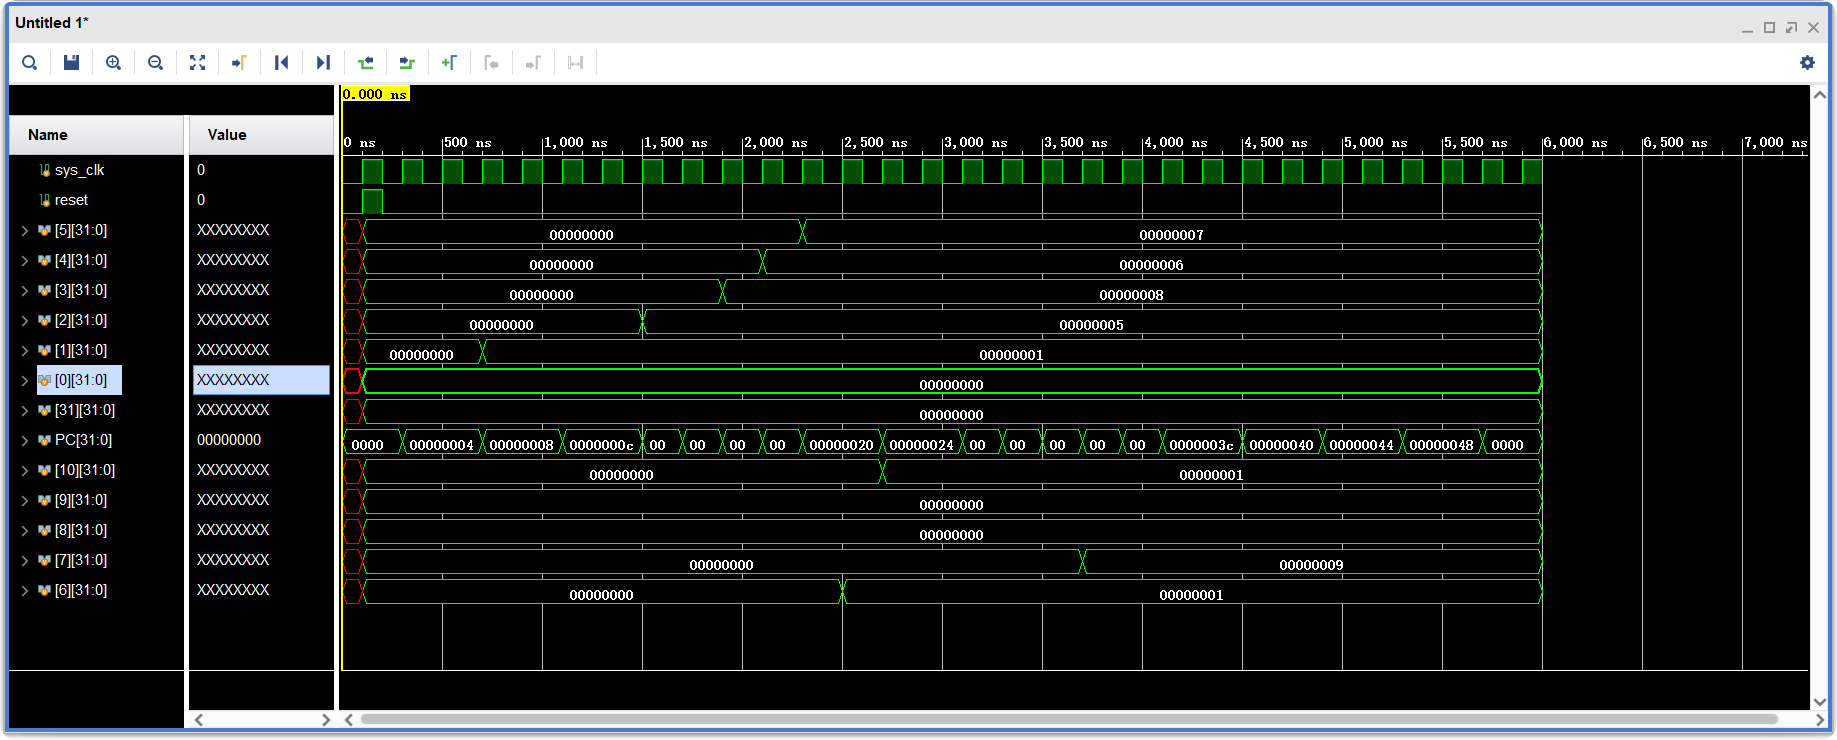
\includegraphics[width=0.98\textwidth]{lab6_final.png}
  \caption{基础流水综合测试最终波形}
  \label{fig:final}
\end{figure}

\subsection{Forwarding 验证波形}

图~\ref{fig:forward} 用于观察普通数据相关场景。波形中寄存器值在连续周期内发生变化，PC 持续推进，没有因为普通 ALU 相关而插入大量停顿。若 Forwarding 失效，后续相关指令会读取旧寄存器值，常见表现是 \$3、\$4 等中间结果错误，且错误会继续传播到后续寄存器。从图中可以看到，相关寄存器最终能够得到正确值，说明 EX/MEM 和 MEM/WB 到 EX 的前递路径能够覆盖相邻指令和间隔一条指令的数据相关。该测试也说明 Forwarding Unit 的优先级处理是必要的：当两个后级同时可能写同一寄存器时，应选择更靠EX的结果。

\begin{figure}[H]
  \centering
  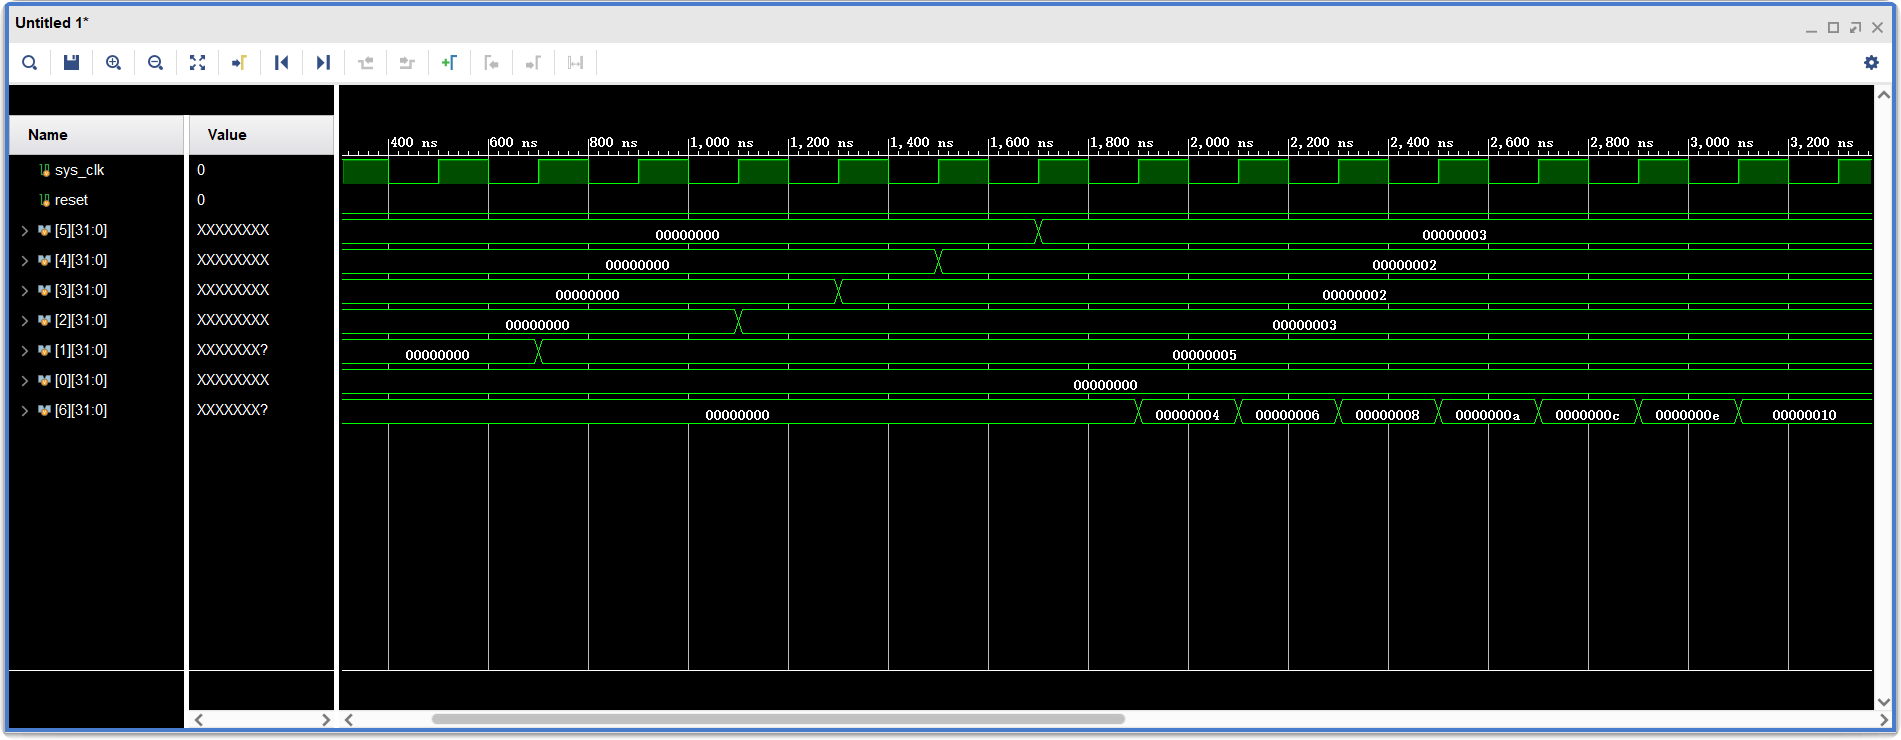
\includegraphics[width=0.95\textwidth]{lab6_basic_forward.png}
  \caption{Forwarding 机制验证波形}
  \label{fig:forward}
\end{figure}

\subsection{Stall 验证波形}

图~\ref{fig:stall} 展示了 load-use 冒险触发 Stall 的情况。图中 Stall 信号被拉高一个周期，对应 PC 和前级流水寄存器暂停。暂停期间，前级不再取入新指令，ID 阶段当前指令保持不变，EX 阶段插入空操作。
这个波形说明 Hazard Detection Unit 能够识别 \texttt{lw} 后立即使用目标寄存器的情况。Stall 结束后，后续指令继续执行，并能通过写回或前递获得正确数据。若没有停顿，\texttt{lw} 的读数尚未从 MEM 阶段产生，后一条指令会使用错误操作数。

\begin{figure}[H]
  \centering
  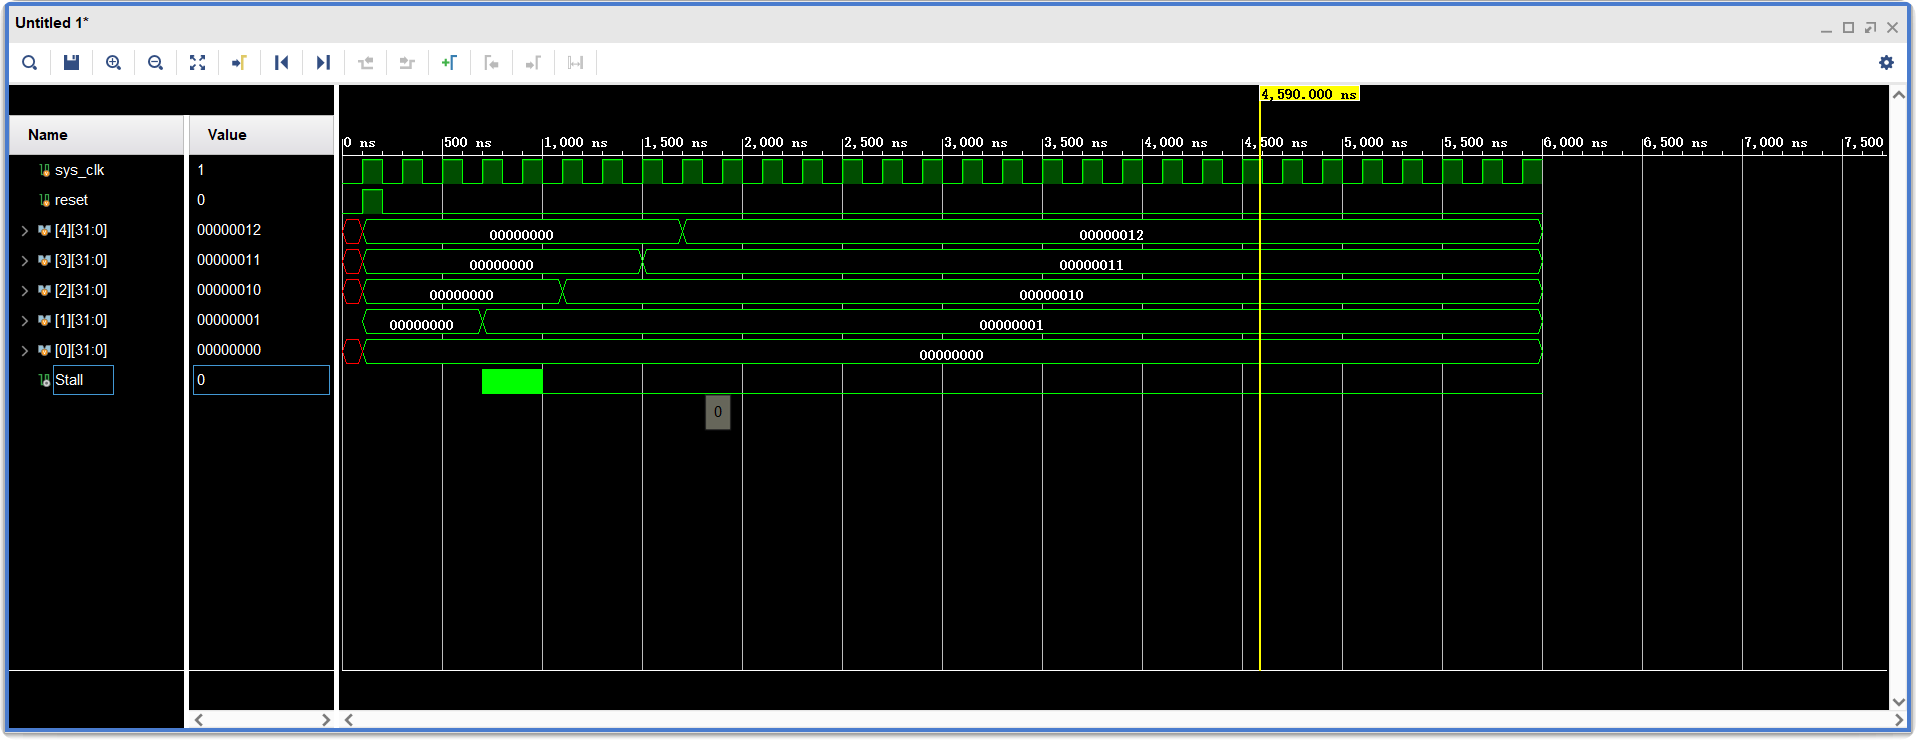
\includegraphics[width=0.95\textwidth]{lab6_stall.png}
  \caption{Stall 机制验证波形}
  \label{fig:stall}
\end{figure}

\subsection{Flush 验证波形}

图~\ref{fig:flush} 为控制冒险处理波形。Flush 信号拉高时，说明当前已经确定需要改变 PC，流水线中顺序取入的指令不再属于正确路径。此时 IF/ID 被清零，PC 改为修正后的目标地址。随后 Flush 信号恢复，流水线从正确地址继续执行。
该图主要验证错误指令是否被清除。如果 Flush 只修改 PC 而不清空 IF/ID，错误路径上的指令仍可能继续进入 EX、MEM、WB 阶段，造成寄存器或内存被错误修改。波形中 Flush 只持续必要周期，后续寄存器结果没有出现异常跳变，说明控制冒险处理有效。

\begin{figure}[H]
  \centering
  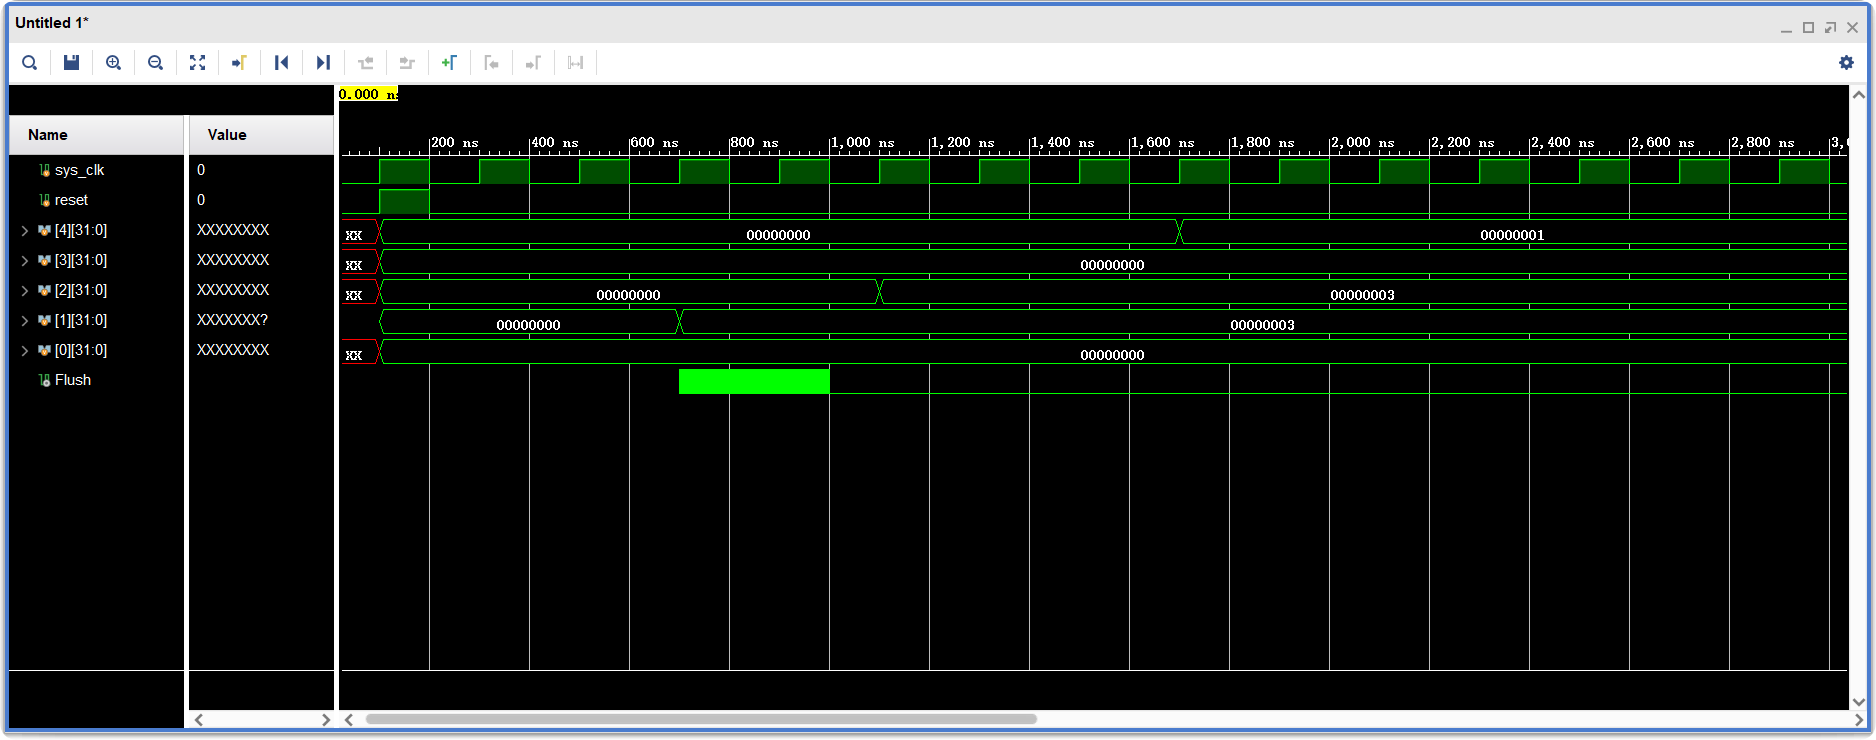
\includegraphics[width=0.90\textwidth]{lab6_flush.png}
  \caption{Flush 机制验证波形}
  \label{fig:flush}
\end{figure}

\subsection{最终波形图}


图~\ref{fig:ext31} 为测试的最终波形。从左侧当前值和波形中的稳定结果可以看到，多个寄存器已经完成更新，说明有符号相关运算、逻辑取反或无符号比较等路径被实际执行到。
该图的意义不只是展示最终几个寄存器值，而是说明整段测试程序能够从 \texttt{jal} 进入、经过多类 ALU/访存/比较/移位指令，再到分支和 \texttt{jr} 控制流位置，整个过程中没有出现 PC 卡死、寄存器异常清零或流水线错误写回等现象。

\begin{figure}[H]
  \centering
  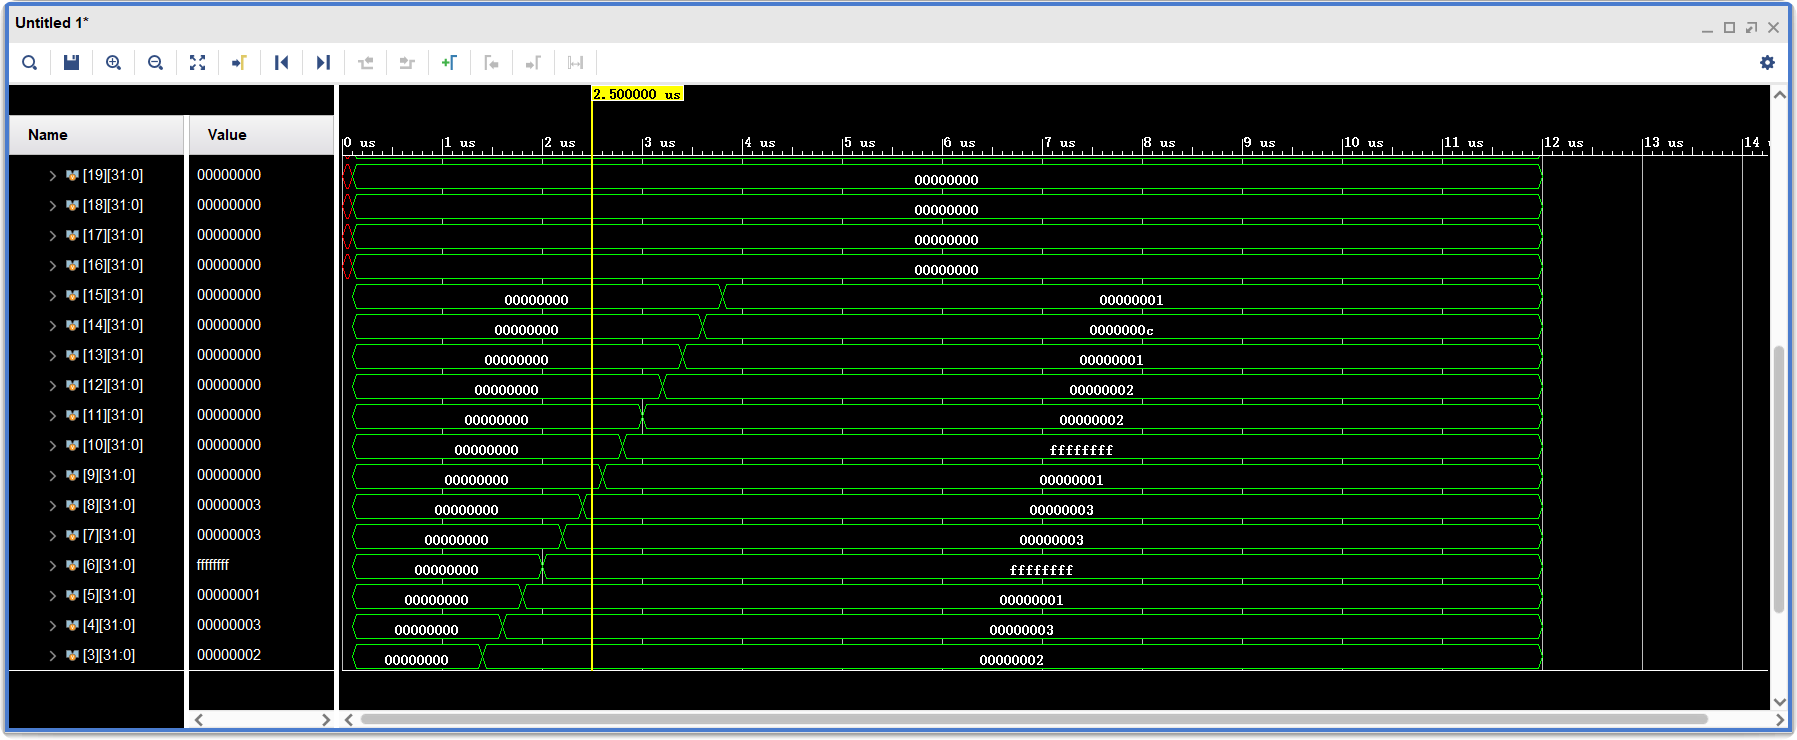
\includegraphics[width=0.90\textwidth]{lab6_31_final.png}
  \caption{测试最终波形}
  \label{fig:ext31}
\end{figure}


\section{31 条指令扩展补充实验}

\subsection{补充实验定位}

31 条指令扩展属于本次 Lab6 的补充实验。前面章节已经验证了基础流水线、Forwarding、Stall 和 Flush 的正确性；本节重点说明在已有流水线框架上如何扩展更多 MIPS 指令，并结合波形说明扩展工程已经跑通。

补充实验与基础实验的关系如下：基础实验保证流水线机制本身正确，31 条指令扩展则要求控制器、ALU 控制器、立即数处理、写回选择和 PC 更新逻辑覆盖更多指令类型。若基础流水机制错误，31 条指令测试中很容易出现连锁错误；若只是个别新增指令译码错误，则通常表现为某个寄存器在对应时间段出现异常结果。因此本节的波形主要用于确认新增指令能够在流水线中顺利执行。

\subsection{扩展指令分类}

本次测试覆盖的指令可以按功能分为几类，如表~\ref{tab:instr31} 所示。

\begin{table}[H]
  \centering
  \caption{31 条指令扩展测试中的主要指令类别}
  \label{tab:instr31}
  \begin{tabular}{p{3.2cm} p{8.7cm}}
    \toprule
    类别 & 测试到的指令及作用 \\
    \midrule
    访存指令 & \texttt{lw}、\texttt{sw}，验证地址计算、数据存储器读写和 \texttt{MemToReg} 写回路径。\\
    算术运算 & \texttt{add}、\texttt{addi}、\texttt{addu}、\texttt{addiu}、\texttt{sub}、\texttt{subu}，验证加减法和有符号/无符号相关译码。\\
    逻辑运算 & \texttt{and}、\texttt{or}、\texttt{xor}、\texttt{nor}、\texttt{ori}、\texttt{xori}，验证 R 型和 I 型逻辑运算路径。\\
    比较指令 & \texttt{slt}、\texttt{sltu}、\texttt{slti}、\texttt{sltiu}，验证有符号和无符号小于比较。\\
    移位指令 & \texttt{sll}、\texttt{srl}、\texttt{sra}、\texttt{sllv}、\texttt{srav}，验证移位量来自 shamt 或寄存器两种情况。\\
    控制流指令 & \texttt{beq}、\texttt{bne}、\texttt{j}、\texttt{jal}、\texttt{jr}，验证 PC 更新、返回地址写入和 Flush。\\
    高位立即数 & \texttt{lui}，验证立即数写入高 16 位的特殊数据通路。\\
    \bottomrule
  \end{tabular}
\end{table}

从实现角度看，扩展指令主要影响三个位置：主控制器需要识别更多 opcode，ALU 控制器需要识别更多 funct，顶层数据通路需要为 \texttt{jal}、\texttt{jr}、\texttt{lui} 和移位类指令提供额外选择。

\subsection{控制器与 ALU 控制器扩展}

主控制器扩展的关键是为不同指令生成正确的控制信号。例如，\texttt{lw} 需要 \texttt{MemRead=1}、\texttt{MemToReg=1}、\texttt{RegWrite=1}；\texttt{sw} 需要 \texttt{MemWrite=1} 且不写寄存器；R 型算术逻辑指令需要 \texttt{RegDst=1}、\texttt{RegWrite=1}，写回数据来自 ALU；I 型立即数指令一般写 \texttt{rt}，第二个 ALU 操作数来自扩展立即数。

\texttt{lui} 和 \texttt{jal} 是两个比较特殊的情况。\texttt{lui} 的结果不是普通符号扩展或零扩展，而是将立即数放到高 16 位；\texttt{jal} 既要改变 PC，又要把返回地址写入 \$31。因此在控制信号中需要额外区分写回目标和写回数据来源。

ALU 控制器扩展时，需要把 R 型指令的 \texttt{funct} 字段映射到不同 ALU 操作。例如 \texttt{xor}、\texttt{nor}、\texttt{sra}、\texttt{sllv}、\texttt{srav} 等都不能复用简单的 add/sub 逻辑。I 型逻辑指令还需要根据 opcode 直接指定 ALU 操作。

\begin{lstlisting}[language=Verilog]
// 示例：根据 ALUOp/funct/opcode 选择 ALU 操作，具体编码以工程实现为准
case (alu_op)
  ALU_OP_RTYPE: begin
    case (funct)
      6'b100000: alu_ctr = ALU_ADD;
      6'b100010: alu_ctr = ALU_SUB;
      6'b100100: alu_ctr = ALU_AND;
      6'b100101: alu_ctr = ALU_OR;
      6'b100110: alu_ctr = ALU_XOR;
      6'b100111: alu_ctr = ALU_NOR;
      6'b000000: alu_ctr = ALU_SLL;
      6'b000010: alu_ctr = ALU_SRL;
      6'b000011: alu_ctr = ALU_SRA;
      6'b000100: alu_ctr = ALU_SLLV;
      6'b000111: alu_ctr = ALU_SRAV;
      default:   alu_ctr = ALU_ADD;
    endcase
  end
endcase
\end{lstlisting}

这里的代码只表示设计思路。实际工程中只要 ALU 控制编码与 ALU 内部实现保持一致即可。

\subsection{立即数与移位类指令处理}

31 条指令扩展中，立即数处理比基础指令更多。\texttt{addi}、\texttt{addiu}、\texttt{slti}、\texttt{sltiu} 使用符号扩展；\texttt{andi}、\texttt{ori}、\texttt{xori} 使用零扩展；\texttt{lui} 需要把低 16 位立即数左移 16 位。若扩展方式错误，寄存器中会出现明显不符合预期的高位数据。

移位类指令也分为两种。\texttt{sll}、\texttt{srl}、\texttt{sra} 使用指令中的 shamt 字段作为移位量；\texttt{sllv}、\texttt{srav} 使用寄存器中的低位作为移位量。因此 ALU 第一个输入或单独的 shamt 输入需要能够在这两种来源之间选择。

\begin{lstlisting}[language=Verilog]
assign shamt_value = use_reg_shamt ? EX_reg_data_1[4:0] : EX_shamt;
assign imm_ext = lui ? {ID_instr[15:0], 16'b0} :
                 sign_ext ? sign_ext_data : zero_ext_data;
\end{lstlisting}

这部分调试时主要观察 \$1、\$2、\$3 等寄存器的变化，因为测试程序中多条移位和立即数指令都写这些寄存器。

\subsection{31 条指令测试程序}

本次补充实验使用的汇编测试程序如下。程序开头先执行 \texttt{jal label} 跳入主体测试段，中间依次测试访存、算术、逻辑、移位、比较和分支，最后通过 \texttt{jr \$ra} 返回。由于 \texttt{lui} 和 \texttt{j end} 位于 \texttt{jal} 后的顺序路径上，它们也可以用于观察跳转和 Flush 是否按预期处理。

\begin{lstlisting}[language={}]
start:
    jal label
    lui $2, 12345
    j end

label:
    lw $1, 8($0)
    lw $1, 12($0)
    lw $2, 16($0)
    add $3, $1, $2
    and $3, $1, $2
    addi $3, $0, 6
    sub $4, $1, $2
    sll $1, $1, 1
    sll $3, $3, 3
    or $1, $3, $1
    addiu $2, $0, 6
    slti $1, $1, 1
    ori $1, $2, 1
    sllv $1, $3, $2
    addu $3, $1, $2
    sub $3, $1, $2
    subu $3, $1, $2
    or $3, $1, $2
    xor $3, $1, $2
    nor $3, $1, $2
    slt $3, $1, $2
    sra $1, $1, 1
    sw $2, 4($0)
    sltu $1, $0, $2
    srl $2, $2, 2
    srav $2, $2, $2
    xori $2, $2, 2
    sltiu $1, $2, 4
    beq $5, $0, label1
    bne $5, $0, label2

label1:
    jr $ra

label2:
    xor $1, $1, $1
    addi $1, $1, 666
\end{lstlisting}

这段程序中，多个指令连续写 \$1、\$2、\$3，可以检查写回目标选择是否正确；多条指令读前面刚写入的寄存器，可以检查 Forwarding 是否仍然适用于扩展指令；\texttt{beq}、\texttt{bne}、\texttt{jal}、\texttt{jr} 则用于检查控制流相关处理。

\subsection{31 条指令波形一：程序进入主体测试段}

图~\ref{fig:ext31-stage1} 为 31 条指令测试的第一段波形。复位结束后，PC 从 0 开始工作。开头执行 \texttt{jal label} 后，程序进入 label 对应的主体测试段。图中可以看到寄存器由未知或 0 状态逐渐被写入有效值，说明取指、跳转、写回路径已经开始正常工作。

这一段主要验证控制流入口是否正确。如果 \texttt{jal} 没有正确跳转，后续会顺序执行 \texttt{lui} 和 \texttt{j end}，主体测试段不会按预期执行；如果 \texttt{jal} 没有正确写 \$31，后面的 \texttt{jr \$ra} 返回也会异常。从波形中 PC 能够继续进入后续测试过程来看，程序入口和返回地址相关逻辑基本正确。

\begin{figure}[H]
  \centering
  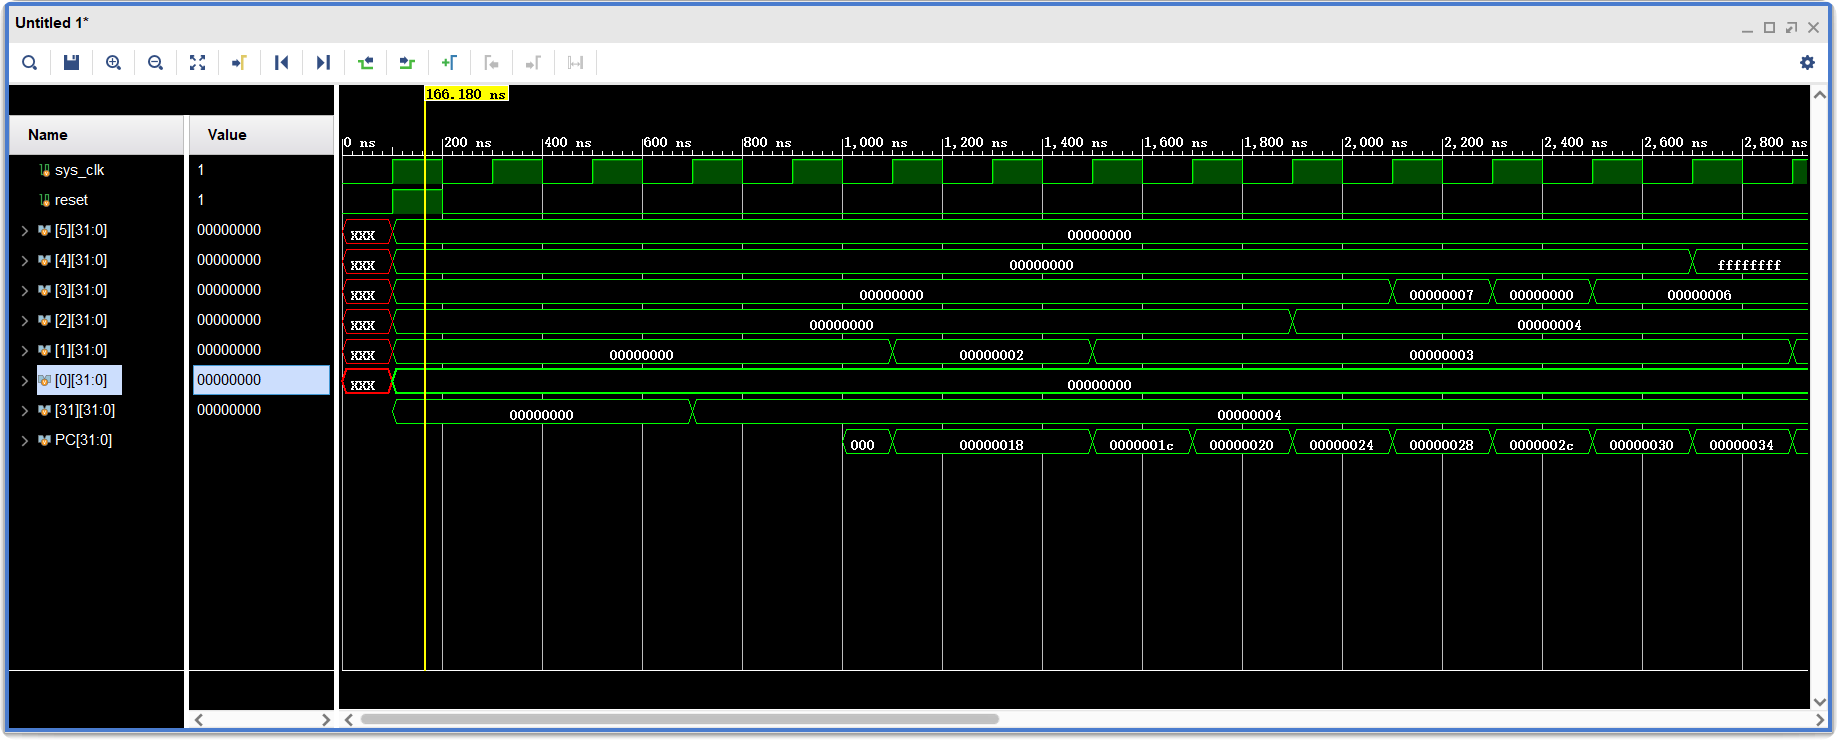
\includegraphics[width=0.98\textwidth]{lab6_31_wave1.png}
  \caption{31 条指令扩展测试波形（一）}
  \label{fig:ext31-stage1}
\end{figure}

\subsection{31 条指令波形二：算术逻辑与移位指令执行过程}

图~\ref{fig:ext31-stage2} 展示了测试程序中部的局部波形。该阶段主要经过 \texttt{add}、\texttt{and}、\texttt{addi}、\texttt{sub}、\texttt{sll}、\texttt{or}、\texttt{addiu}、\texttt{slti}、\texttt{ori} 等指令。可以看到 PC 按 4 字节对齐地址不断推进，同时 \$1、\$2、\$3、\$4 等寄存器在不同周期被更新。

波形中出现的 \texttt{00000006}、\texttt{00000007}、\texttt{00000030}、\texttt{ffffffff} 等值，分别对应立即数赋值、逻辑运算、移位结果或有符号减法/取反类结果。这说明 ALU 控制器已经能够区分多种操作，而不是只执行基础的加法或减法。该段还可以间接说明 Forwarding 对扩展指令依然有效，因为测试程序中存在连续写读同一寄存器的情况。

\begin{figure}[H]
  \centering
  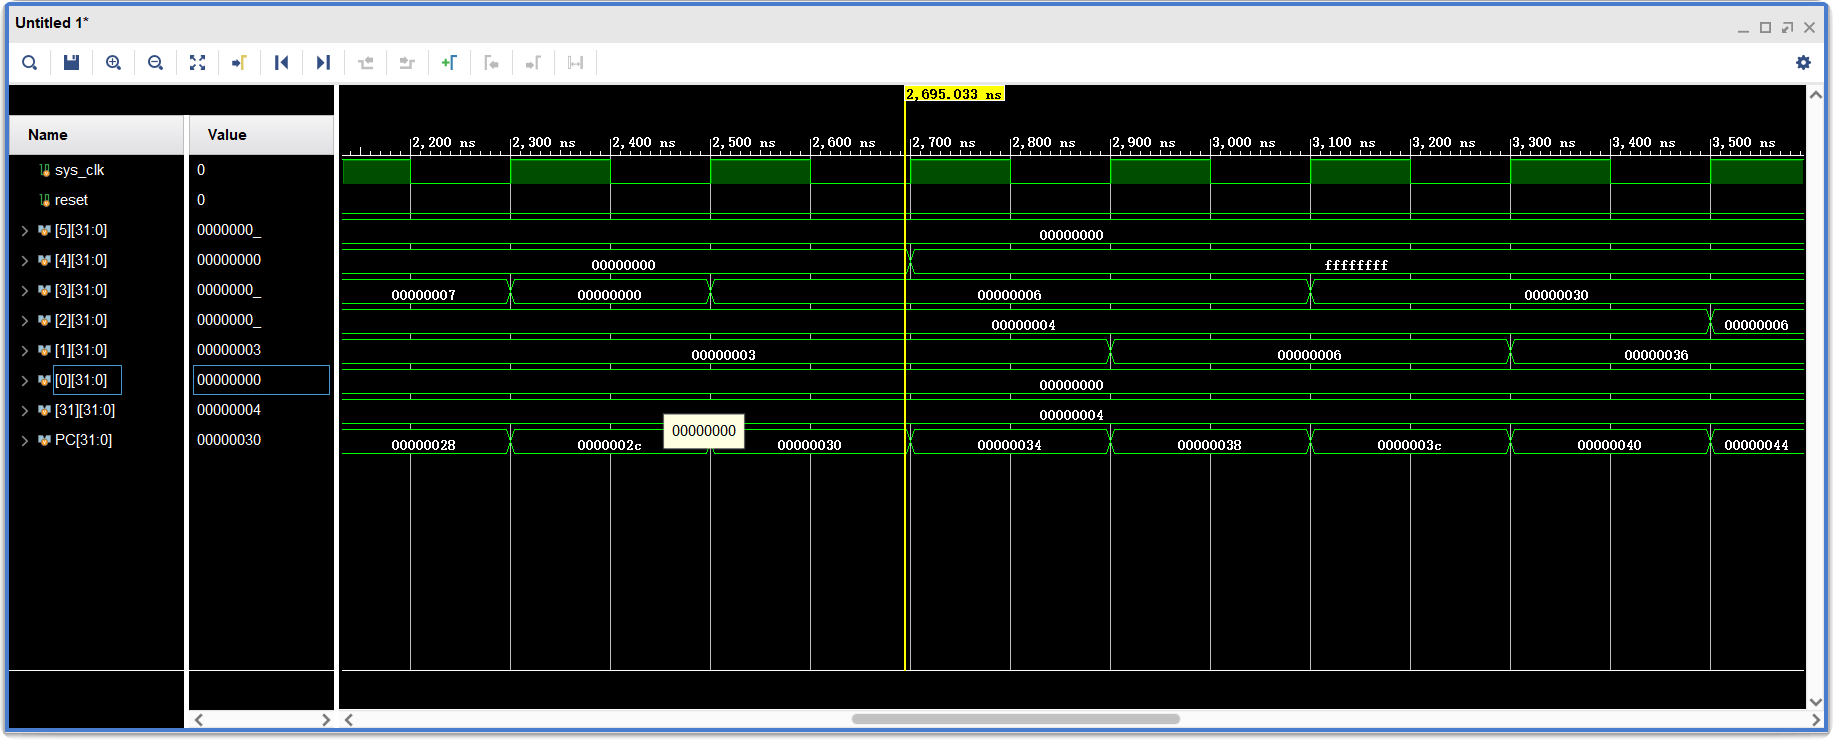
\includegraphics[width=0.98\textwidth]{lab6_31_wave2.png}
  \caption{31 条指令扩展测试波形（二）}
  \label{fig:ext31-stage2}
\end{figure}



\section{实现过程中的问题分析}

\subsection{控制信号与指令错位}

流水线 CPU 中，控制信号在 ID 阶段生成，但其真正发挥作用的位置可能在 EX、MEM 或 WB 阶段。因此，控制信号必须和对应指令一起写入流水寄存器并逐级传递。如果后级直接使用当前 ID 阶段新生成的控制信号，就会导致控制信号与数据不属于同一条指令，从而出现错误写回、错误访存等问题。

本实验中，ID/EX、EX/MEM 和 MEM/WB 流水寄存器都需要保存对应阶段后续会使用的控制信号。例如 RegWrite、MemRead、MemWrite、MemToReg 等信号不能只在 ID 阶段临时生成，而应随指令向后传播。这样才能保证 WB 阶段写回的目标寄存器和写回数据仍然对应同一条指令。

\subsection{Forwarding 优先级问题}

Forwarding 的判断不仅要检测寄存器号是否相同，还要处理优先级。当 EX/MEM 和 MEM/WB 阶段都可能向当前 EX 阶段前递同一个寄存器时，应优先选择 EX/MEM 阶段的数据，因为它来自距离当前指令更近的一条指令，代表更新的结果。

若优先级处理不当，连续写同一寄存器时可能会取到较旧的 WB 阶段数据。为避免这一问题，Forwarding Unit 中先判断 EX/MEM 前递条件，再判断 MEM/WB 前递条件，并在 MEM/WB 判断时排除 EX/MEM 已命中的情况。

\subsection{Stall 处理不完整}

load-use 冒险不能仅靠 Forwarding 解决，因为 lw 指令的数据需要到 MEM 阶段后才可获得。检测到 load-use 冒险后，Stall 需要同时作用于 PC、IF/ID 和 ID/EX 三个位置：PC 保持不变，IF/ID 保持当前指令，ID/EX 插入空操作。

如果只暂停 PC，IF/ID 中的指令仍可能变化；如果只暂停前级而不清空 ID/EX 控制信号，错误指令仍可能进入 EX 阶段执行。因此 Stall 的关键不是单纯“停一个周期”，而是要让前级保持、后级插入 bubble。

\subsection{Flush 只修改 PC 不够}

控制冒险处理中，分支或跳转确定后需要更新 PC，但仅修改 PC 不能完全消除错误路径指令。因为在 PC 修正前，流水线中可能已经顺序取入了错误指令，如果这些指令继续向后传播，就可能产生错误写回或错误访存。

因此 Flush 需要和 IF/ID 流水寄存器配合，将错误取入的指令清零。这样即使错误路径上的指令已经进入前级，也不会在后续阶段产生有效控制信号。

\section{实验总结}

本次实验完成了类 MIPS 五级流水 CPU 的设计、冒险处理和补充指令扩展验证。相比 Lab5 的单周期 CPU，流水线 CPU 的核心难点在于同一时刻存在多条指令，必须明确每个信号属于哪一条指令、哪一个流水阶段。通过加入四组流水寄存器，处理器能够把数据和控制信号稳定传递到后级；通过 Forwarding，普通 RAW 数据相关可以在不暂停流水线的情况下被解决；通过 Stall，load-use 冒险能够通过插入一个 bubble 保证正确性；通过 Flush，控制流改变后错误路径指令不会继续产生副作用。

从仿真结果看，基础流水测试能够得到正确寄存器结果，Forwarding、Stall 和 Flush 在对应波形中均有明确体现。31 条指令扩展作为补充实验，也通过测试程序和三张波形展示了新增算术逻辑、立即数、移位、比较、访存和控制流指令的执行过程。总体来看，本次实验已经完成基础要求和 31 条指令补充验证。

总的来说，这六个实验循序渐进还可以复用模块让我对CPU的架构又一次得到了深刻的认识与理解。感谢一直细心讲解的苏老师，还有遇到问题给我提供详细讲解的三位助教们！

\end{document}
